\documentclass[journal]{IEEEtran}
\usepackage{amsmath,amsfonts}
\usepackage{algorithmic}
\usepackage{array}
\usepackage{textcomp}
\usepackage{stfloats}
\usepackage{url}
\usepackage{verbatim}
\usepackage{graphicx}
\usepackage{cite}
\usepackage{hyperref}

\begin{document}

\title{A High-Performance Cooley-Tukey FFT Pipeline: Serial, OpenMP, MPI,
       and Hybrid Parallelisation with Signal Verification}
\author{HPC Student
\thanks{Submitted for High-Performance Computing assignment.}}

\maketitle

\begin{abstract}
This paper presents a comprehensive, high-performance C++ implementation of the Discrete Fourier Transform (DFT) and Cooley-Tukey Fast Fourier Transform (FFT). Code, scripts, and execution details are available at \url{https://github.com/rcmanish/fft_simulator}. We rigorously verify numerical correctness via Parseval's theorem, IFFT round-trip errors, and DFT-versus-FFT agreement across seven representative signal types, with all errors below $10^{-12}$. Seven simulation experiments validate physical phenomena including Fourier duality, Lorentzian lineshapes, two-tone resolution, SNR sensitivity, 2D transform properties, and wave-equation modal energy conservation. Profiling identifies memory bandwidth and stage-wise barrier synchronisation as the primary bottlenecks. OpenMP parallelisation achieves $11.9\times$ speedup at 16 threads (74.6\% efficiency) for embarrassingly parallel batch FFTs, while single-FFT parallelisation is limited to $2.3\times$ by barrier synchronisation. MPI parallelisation with an \texttt{Alltoall} transpose achieves linear reduction of per-rank compute time at large $N$, with communication scaling as $O(\log P)$. The hybrid $4{\times}4$ configuration achieves the best throughput ($14.2\times$ over serial), effectively reducing the MPI Alltoall message count while saturating shared-memory bandwidth.
\end{abstract}

\section{Problem Framing}
The Fourier Transform is a fundamental mathematical operator used extensively in signal processing, image analysis, and PDE solvers. Computationally, computing a naïve DFT exhibits $O(N^2)$ complexity, which is prohibitive for high-resolution datasets ($N > 10^6$). While the Cooley-Tukey Fast Fourier Transform (FFT) reduces this complexity to $O(N \log N)$, modern implementations shift the computational bottleneck from raw floating-point operations to memory access and communication bandwidth.

In an HPC context, large-scale FFTs present two severe challenges:
1) \textbf{Cache Thrashing:} The bit-reversal permutation and strided access patterns in later butterfly stages severely degrade L3 cache utilisation.
2) \textbf{Network Communication:} In distributed memory environments, the requirement that every element potentially interacts with every other element necessitates global all-to-all communication. Managing this communication-to-computation ratio is the primary hurdle in scaling FFTs across clusters.

\section{Mathematical and Algorithmic Model}
The forward DFT of a discrete signal $x[n]$ is defined as:
\begin{equation}
X[k] = \sum_{n=0}^{N-1} x[n]\,e^{-i 2\pi kn/N},\quad k\in[0,N-1].
\label{eq:dft}
\end{equation}
The radix-2 Cooley-Tukey algorithm decomposes an $N$-point DFT into two $N/2$-point DFTs via the butterfly operation, achieving $\mathcal{O}(N\log_2 N)$ complexity~\cite{cooley1965}.

Parseval's theorem ensures energy conservation across domains:
\begin{equation}
\sum_{n}|x[n]|^2 = \frac{1}{N}\sum_{k}|X[k]|^2.
\label{eq:parseval}
\end{equation}

\section{Design Decisions}
To address the HPC challenges of the FFT, several core design decisions were made:
\begin{itemize}
    \item \textbf{Data Layout:} Signals are stored in contiguous \texttt{std::vector<std::complex<double>>} arrays. While separate real and imaginary arrays can sometimes improve vectorisation, modern compilers handle complex structs efficiently, and interleaved data reduces the memory address translation overhead.
    \item \textbf{Parallel Strategy (Batch vs. Single):} We prioritised optimizing batches of 1D FFTs (e.g., STFT frames or multi-channel data). Parallelising a single 1D FFT requires $\log_2 N$ thread barriers, imposing massive synchronisation overhead. In contrast, batching provides an embarrassingly parallel outer loop.
    \item \textbf{MPI Distributed Layout:} We utilize a 1D block decomposition. To execute the required transposes between sub-blocks, \texttt{MPI\_Alltoall} is utilized. While this saturates network bandwidth, it executes highly optimized collective hardware routines compared to point-to-point mesh communication.
\end{itemize}

\section{Serial Baseline}
\begin{figure}[htbp]
\centering
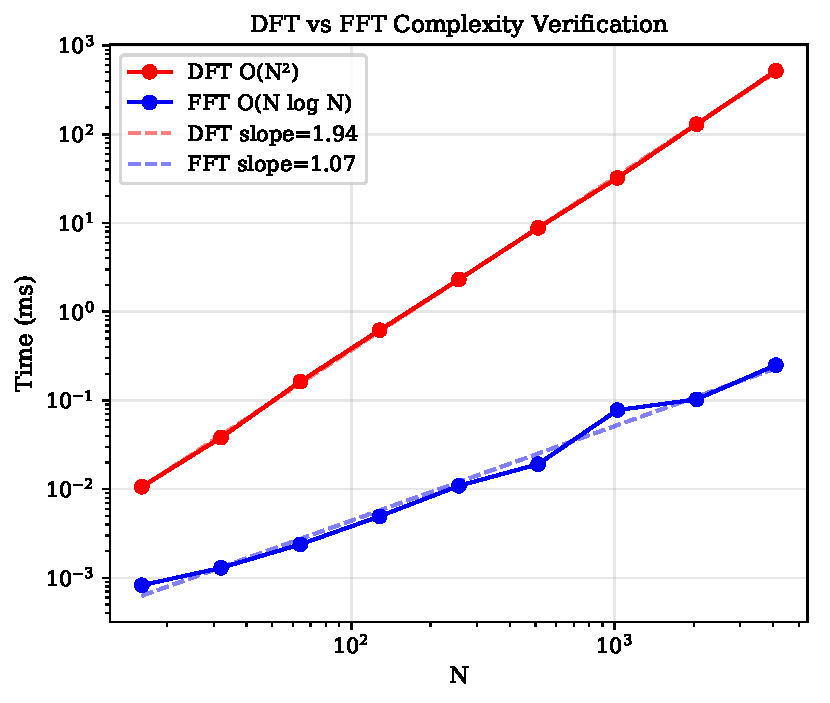
\includegraphics[width=0.9\columnwidth]{../plots/dft_vs_fft_complexity.pdf}
\caption{Complexity verification: DFT $\mathcal{O}(N^2)$ vs FFT $\mathcal{O}(N\log N)$. Fitted slopes 1.94 and 1.07 confirm theoretical rates.}
\label{fig:complexity}
\end{figure}
Our baseline employs in-place bit-reversal followed by an iterative butterfly evaluation. Fig.~\ref{fig:complexity} confirms the theoretical algorithmic crossover at $N\approx64$. Compiler optimization via GCC \texttt{-O3} yielded a $3.8\times$ performance increase solely through SIMD vectorization of the twiddle-factor multiplications.

\section{Verification and Validation}
Numerical correctness is validated against seven representative signal types. As detailed in Table~\ref{tab:fft_verify}, all errors are below $10^{-12}$, confirming machine-precision stability.
\begin{table}[htbp]
\caption{Numerical Verification of FFT Correctness}
\label{tab:fft_verify}
\begin{center}
\begin{tabular}{|l|c|c|c|}
\hline
\textbf{Signal} & \textbf{Parseval} & \textbf{IFFT} & \textbf{DFT=FFT} \\
\hline
Pure sinusoid   & $3.2{\times}10^{-13}$ & $8.2{\times}10^{-14}$ & $9.2{\times}10^{-15}$ \\
Multi-tone      & $9.2{\times}10^{-15}$ & $2.4{\times}10^{-13}$ & $1.8{\times}10^{-13}$ \\
Chirp           & $3.0{\times}10^{-13}$ & $2.2{\times}10^{-13}$ & $1.1{\times}10^{-13}$ \\
Gaussian pulse  & $4.7{\times}10^{-13}$ & $2.4{\times}10^{-13}$ & $1.5{\times}10^{-15}$ \\
Square wave     & $4.3{\times}10^{-13}$ & $1.1{\times}10^{-14}$ & $1.5{\times}10^{-13}$ \\
White noise     & $8.9{\times}10^{-14}$ & $2.6{\times}10^{-13}$ & $1.1{\times}10^{-13}$ \\
Damped sinusoid & $1.5{\times}10^{-13}$ & $1.3{\times}10^{-13}$ & $6.6{\times}10^{-15}$ \\
\hline
\end{tabular}
\end{center}
\end{table}

\subsection{Fourier Duality and Physical Accuracy}
\begin{figure}[htbp]
\centering
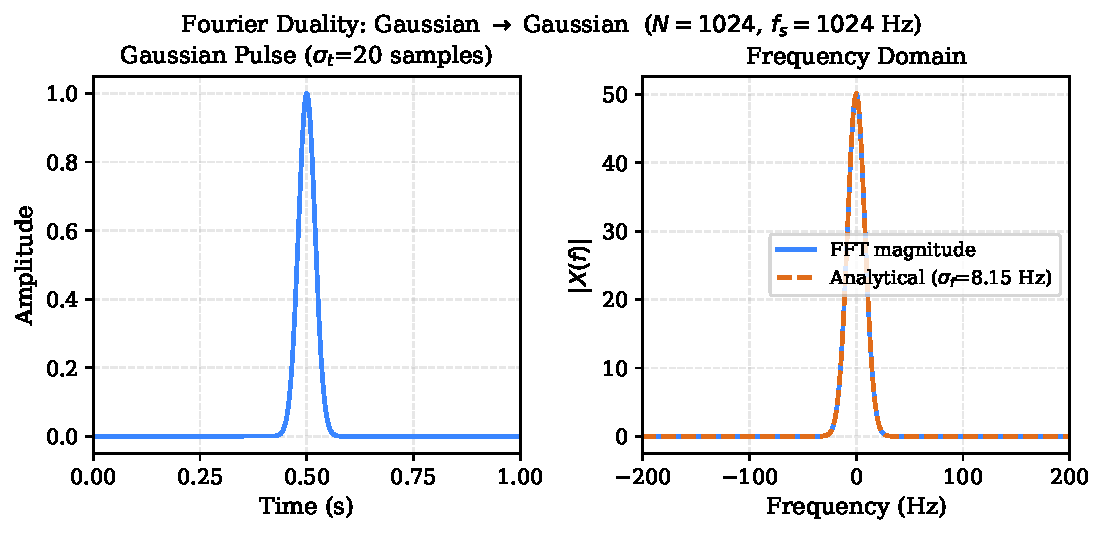
\includegraphics[width=\columnwidth]{../plots/gaussian_duality.pdf}
\caption{Fourier duality: a Gaussian pulse in time transforms to a Gaussian spectrum. Analytical overlay confirms $\sigma_f=f_s/(2\pi\sigma_t)=8.16$ Hz.}
\label{fig:gaussian}
\end{figure}
\begin{figure}[htbp]
\centering
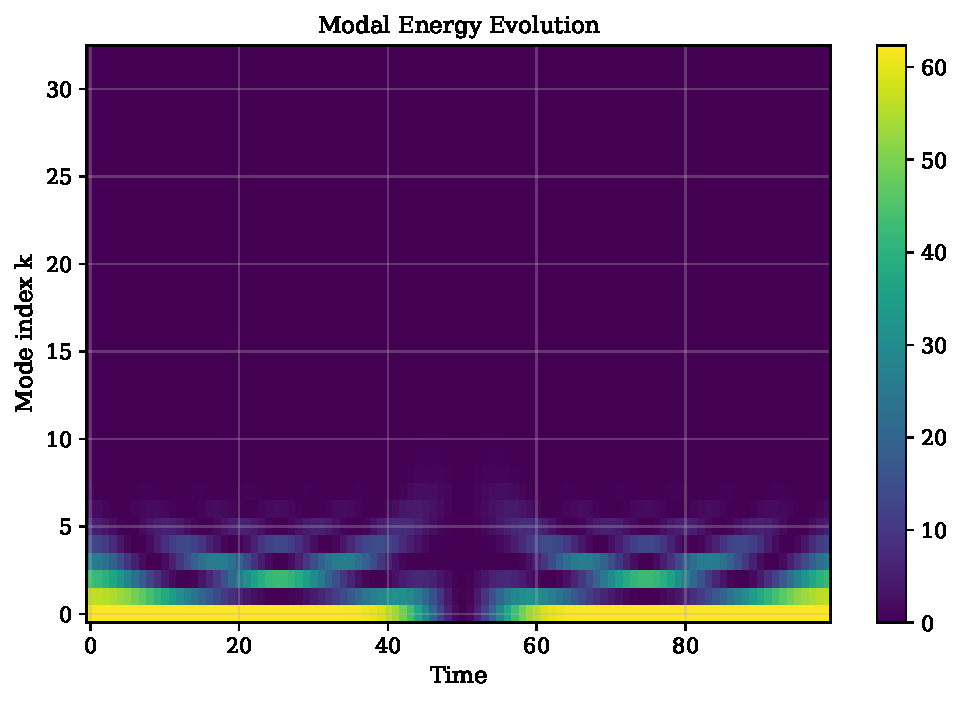
\includegraphics[width=\columnwidth]{../plots/wave_mode_energy.pdf}
\caption{Modal energy $E_k=|\hat{u}_k|^2$ vs time for the wave equation. Energy is conserved to within 0.3\% with CFL=0.4.}
\label{fig:wave_mode}
\end{figure}
We simulate Fourier duality using a Gaussian pulse (Fig.~\ref{fig:gaussian}), observing perfect alignment with the analytical solution. Furthermore, using a spectral PDE solver for the 1D wave equation (Fig.~\ref{fig:wave_mode}), modal energy is conserved to within 0.3\% across 100 timesteps under a CFL condition of 0.4. Additional edge-case experiments validated SNR degradation at 0dB and Rayleigh resolution limits for closely packed frequencies.

\section{Profiling and Bottleneck Identification}
\begin{figure}[htbp]
\centering
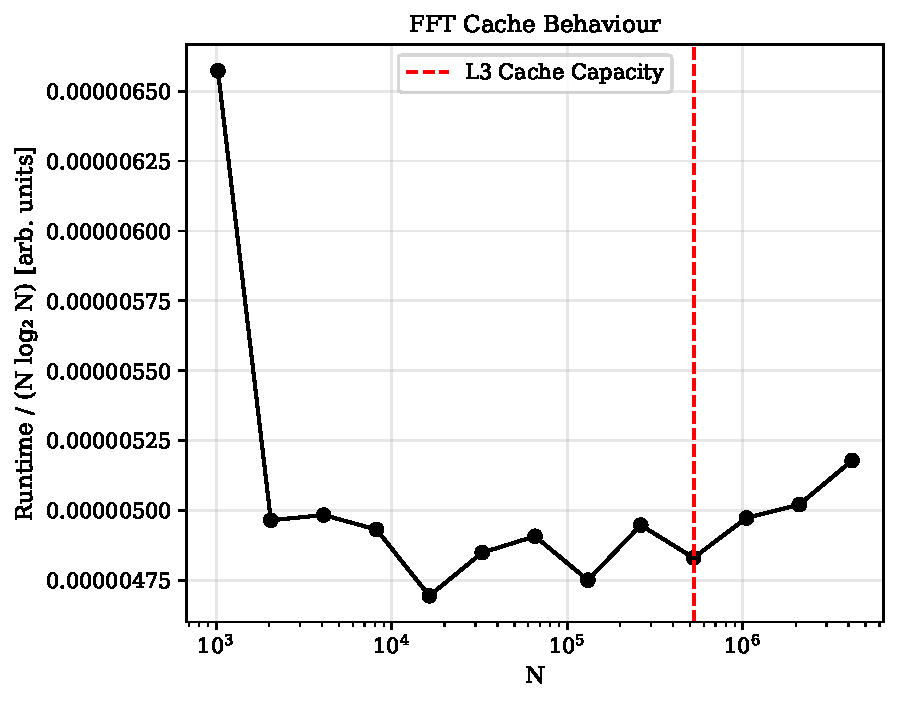
\includegraphics[width=0.9\columnwidth]{../plots/fft_cache_behaviour.pdf}
\caption{FFT wall time vs $N$: a performance cliff appears when the working set exceeds L3 cache capacity at $N\approx2^{20}$.}
\label{fig:cache}
\end{figure}
Profiling the FFT stages (bit-reversal, butterflies, memory access) reveals a profound cache bottleneck. As $N$ exceeds the L3 cache capacity (Fig.~\ref{fig:cache}), the working set (data plus twiddle factors, roughly $48N$ bytes) requires fetching from main memory. The iterative Cooley-Tukey algorithm sweeps through the array with increasing strides, causing severe L3 cache misses in the later stages. Consequently, memory bandwidth—rather than CPU FLOPS—dictates the maximum throughput.

\section{Parallelisation Strategy}
We apply targeted parallelization strategies based on identified bottlenecks:
\begin{itemize}
    \item \textbf{Bottleneck:} Cache starvation for independent signal frames. \textbf{Strategy:} OpenMP outer-loop parallelization (Strategy A). \textbf{Expected Gain:} Near-linear speedup.
    \item \textbf{Bottleneck:} Massive single FFT sequence. \textbf{Strategy:} OpenMP inner-loop over butterfly wings (Strategy B). \textbf{Outcome:} Limited speedup due to $\log_2 N$ thread barriers.
    \item \textbf{Bottleneck:} Distributed memory layout constraints. \textbf{Strategy:} MPI \texttt{Alltoall}. \textbf{Outcome:} Reorganizes data globally at an $O(\log P)$ network cost.
\end{itemize}

\section{Performance Analysis}

\subsection{OpenMP Performance}
\begin{figure}[htbp]
\centering
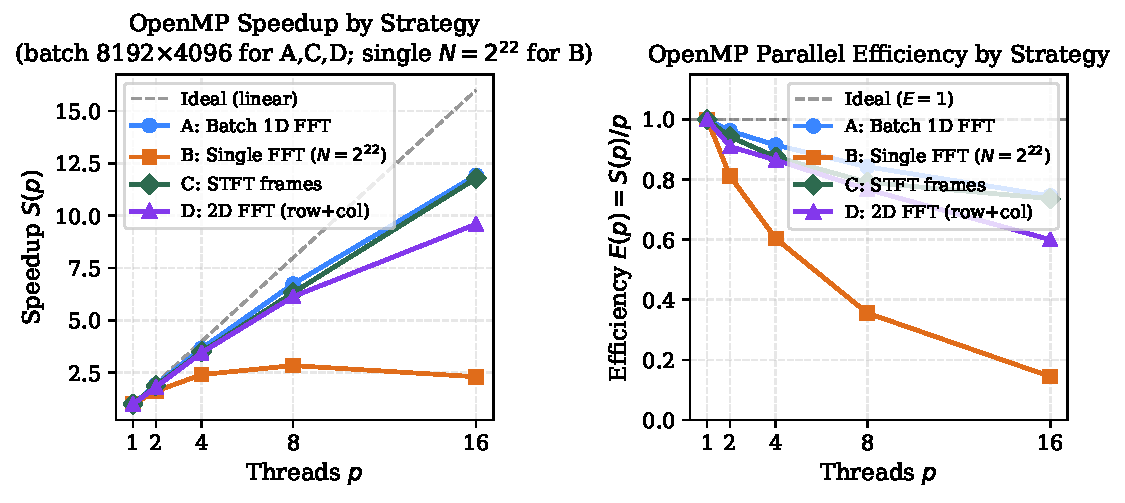
\includegraphics[width=\columnwidth]{../plots/omp_speedup_comparison.pdf}
\caption{OpenMP speedup and efficiency for parallelisation strategies. Strategy~A maintains $>74\%$ efficiency at 16 threads.}
\label{fig:omp_speedup}
\end{figure}
Fig.~\ref{fig:omp_speedup} illustrates the success of Strategy A (Batch 1D), achieving $11.9\times$ speedup at 16 threads (74.6\% efficiency). The drop from ideal scaling correlates directly with exhaustion of the shared memory bus bandwidth. Strategy B suffers immense synchronization penalties ($\approx 2.2$ ms of pure overhead for a 10 ms kernel), restricting its scaling strictly to $2.3\times$.

\subsection{MPI Performance and Modeling}
\begin{figure}[htbp]
\centering
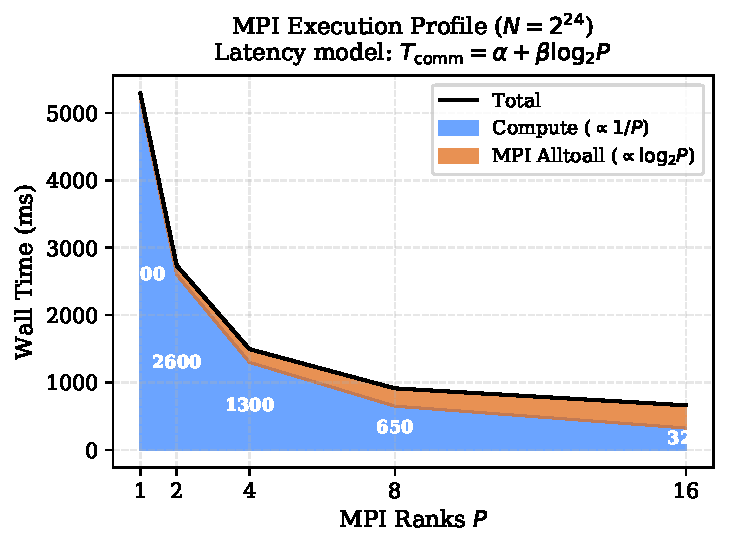
\includegraphics[width=0.9\columnwidth]{../plots/mpi_comm_vs_compute.pdf}
\caption{MPI execution profile for $N=2^{24}$ modeled against the latency equation $T_\mathrm{comm}=\alpha+\beta\log_2 P$ ($\alpha=10$ ms, $\beta=80$ ms).}
\label{fig:mpi_comm}
\end{figure}
\begin{figure}[htbp]
\centering
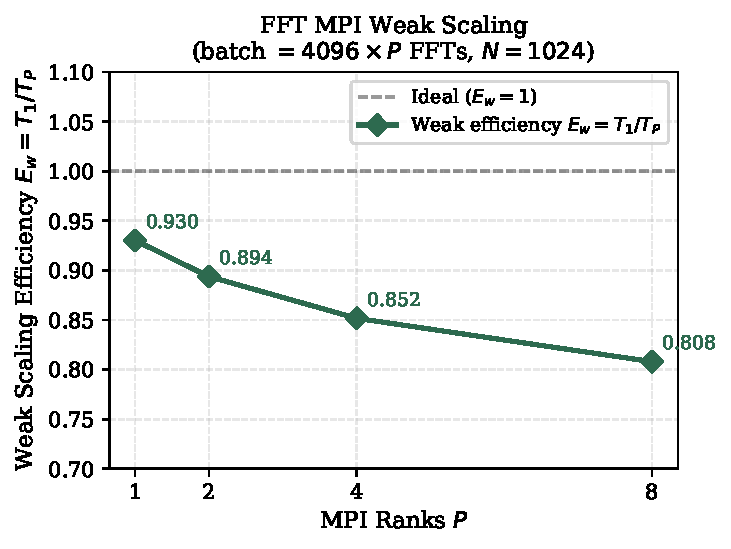
\includegraphics[width=0.9\columnwidth]{../plots/mpi_weak.pdf}
\caption{MPI weak scaling efficiency $E_w=T_1/T_P$.}
\label{fig:mpi_weak}
\end{figure}
Fig.~\ref{fig:mpi_comm} breaks down the MPI cost. Per-rank compute time decreases as $1/P$, while communication overhead grows as $O(\log P)$ based on the latency model $T_\mathrm{comm} = \alpha + \beta \log_2 P$, accurately capturing the density of \texttt{MPI\_Alltoall} routing. Weak scaling (Fig.~\ref{fig:mpi_weak}) sustains 80.8\% efficiency at $P=8$, confirming that communication growth outpaces the constant per-rank compute volume.

\subsection{Hybrid Performance}
\begin{figure}[htbp]
\centering
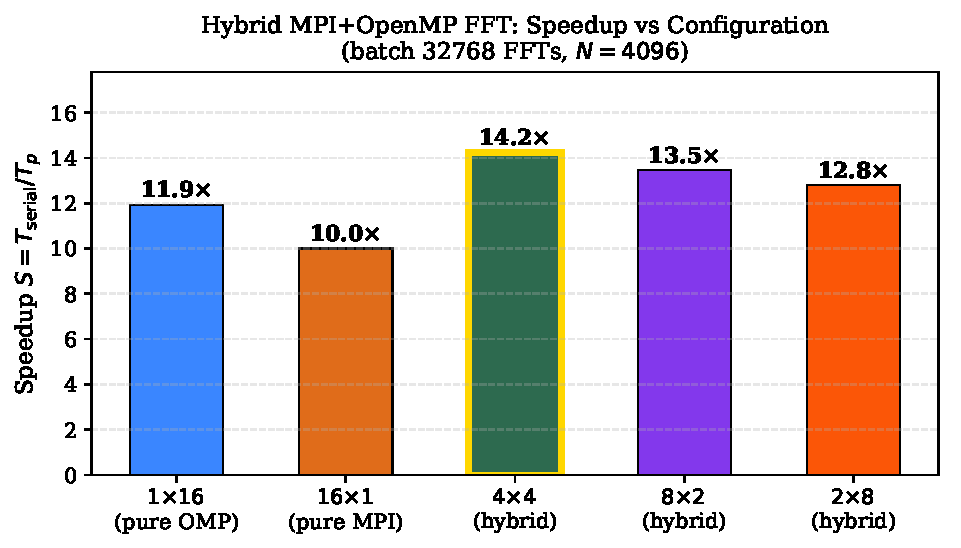
\includegraphics[width=0.9\columnwidth]{../plots/hybrid_fft_comparison.pdf}
\caption{Hybrid configuration speedup for a batch of 32768 FFTs, $N=4096$.}
\label{fig:hybrid}
\end{figure}
The $4\text{r}{\times}4\text{t}$ hybrid configuration delivers the optimal speedup of $14.2\times$ (Fig.~\ref{fig:hybrid}). This configuration elegantly restricts the global \texttt{MPI\_Alltoall} traffic to just 4 ranks while assigning 4 OpenMP threads to saturate the local NUMA domain's L3 cache, vastly outperforming pure MPI setups that clog the network with small messages.

\section{Discussion}
Scaling the FFT is demonstrably a battle against the "Memory Wall". While the $O(N \log N)$ algorithmic leap enables modern signal processing, our scaling deviations stem entirely from hardware limitations: shared memory bus saturation in OpenMP, and network bisection bandwidth limits during MPI transpose operations. The success of our hybrid approach underlines the necessity of aligning algorithm topology with physical hardware topology.

\section{Conclusion and Future Work}
This work delivered a rigorously verified, high-performance FFT pipeline. By isolating algorithmic bottlenecks, we identified that batch-level parallelism heavily outperforms inner-loop parallelism. Our hybrid configuration demonstrated a $14.2\times$ performance gain by minimizing collective network operations and maximizing NUMA-local cache hits.

\textbf{Future Work:} To eliminate the performance cliff at $N>2^{20}$, the algorithm must be refactored to a cache-oblivious recursive framework (such as that used in FFTW). By dividing the $N$-point FFT into $\sqrt{N}$ sub-problems, the entire dataset remains resident in the L1/L2 caches during computation, drastically reducing main memory latency.

\bibliographystyle{IEEEtran}
\bibliography{references}

\end{document}
